\chapter{الفئة p \texorpdfstring{\babelsublr{(2)}}{(2)}: الأكسجين والهالوجينات والغازات النبيلة}\label{ch:b1:p-block-16-18}

يُصنع حمض الكبريتيك بحمولة تفوق أي مادة كيميائية أخرى: فهو
يذيب صخر الفوسفات من أجل الأسمدة، ويرشّح خامات النحاس واليورانيوم،
ويكرّر النفط ويملأ بطاريات السيارات، وطوال قرن كان إنتاج
حمض الكبريتيك مقياسًا تقريبيًا لصناعة البلد. ويأتي معظم كبريته
اليوم من تنقية الغاز الطبيعي والنفط؛ وما زال بعضه يُحمل باليد
من فوهات البراكين. ويقع الكبريت في \omterm{def:b1:periodicity:table}{الزمرة} 16 تحت
الأكسجين؛ وتُكمل هالوجينات \omterm{def:b1:periodicity:table}{الزمرة} 17 والغازات النبيلة في \omterm{def:b1:periodicity:table}{الزمرة} 18
\omterm{def:b1:periodicity:table}{الفئة} p. يتتبع هذا الفصل الأكسجين والكبريت من العنصر إلى
الحمض، ويرتّب \omterm{def:b1:p-block-16-18:halogen}{الهالوجينات} مؤكسداتٍ بجهودها المعيارية،
وينتهي بالمركبات التي تكوّنها فعلًا الغازات النبيلة المفترض أنها خاملة.

\begin{recall}
\omterm{def:b1:lewis-resonance-vsepr:lewis}{بنى لويس}، والثمانيات الموسَّعة وأشكال VSEPR (\cref{ch:b1:lewis-resonance-vsepr})؛
\omterm{def:b1:nernst:electrode-potential}{والجهود المعيارية} (\cref{ch:b1:nernst})؛ \omterm{def:b1:e-ph-diagrams:disproportionation}{وعدم تناسب}
الكلور \omterm{def:b1:e-ph-diagrams:e-ph-diagram}{ومخطط الجهد--pH} للكلور
(\cref{ch:b1:e-ph-diagrams})؛ والحفز (\cref{ch:b1:elementary-steps}).
وقد جمع المجلد المدرسي (الصف العاشر) \omterm{def:b1:p-block-16-18:halogen}{الهالوجينات} والغازات النبيلة في
عائلات.
\end{recall}

\begin{omfigure}
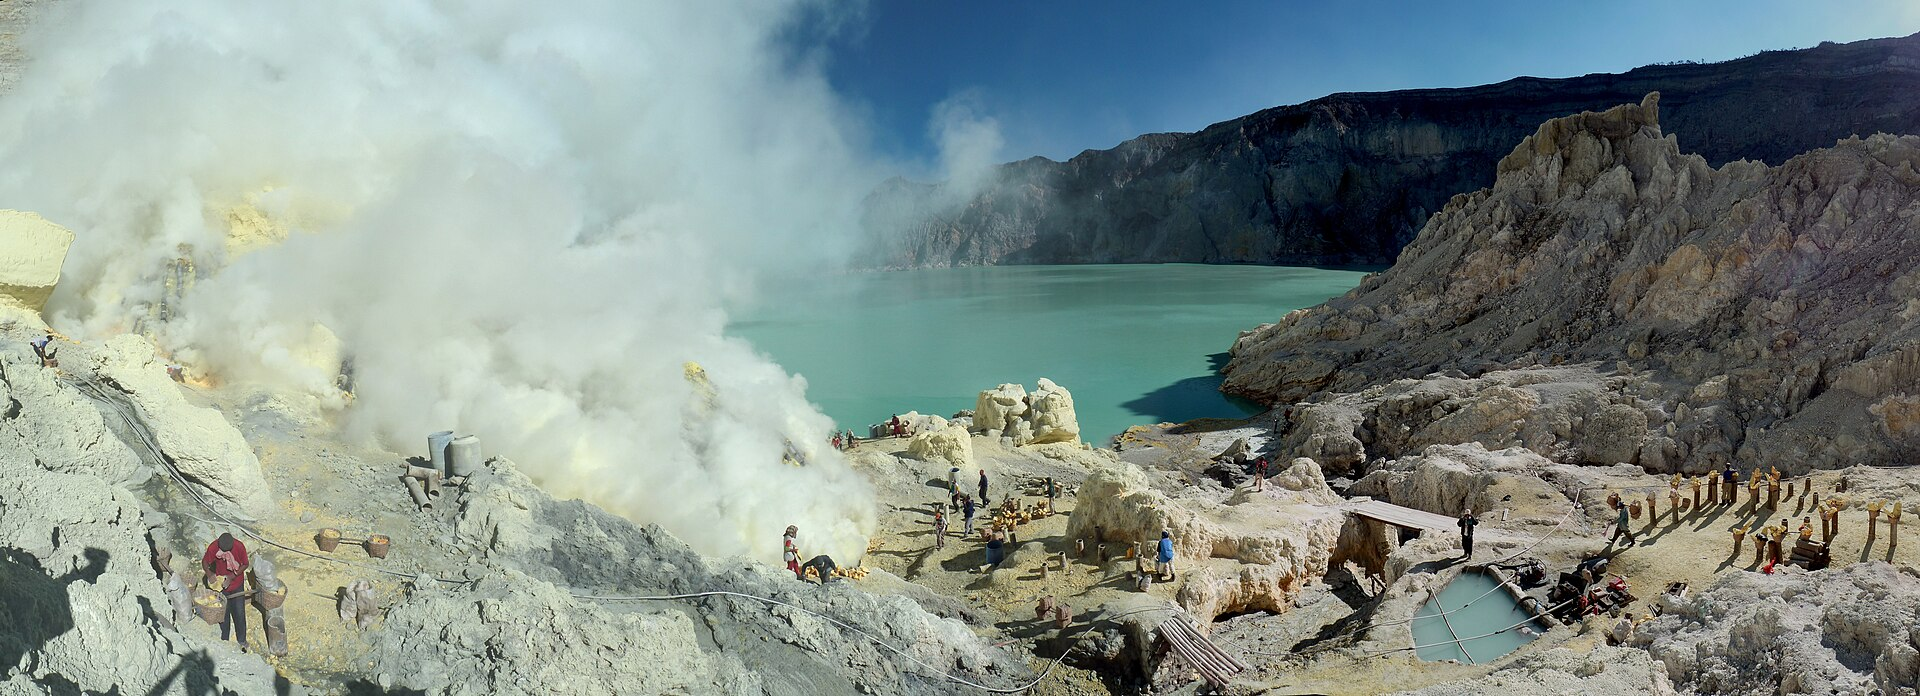
\includegraphics[width=0.78\linewidth]{images/book2/kawah-ijen.jpg}

{\small استخراج الكبريت في فوهة بركان كاوا إيجين، إندونيسيا:
تكثّف الغازات البركانية الكبريت الأصفر حول الأنابيب، ويحمله العمال
إلى الخارج في سلال (صورة سيمور، CC BY-SA 4.0، ويكيميديا كومنز).}
\end{omfigure}

\section{الأكسجين والأوزون وفوق الأكاسيد}

\begin{definition}[الكالكوجينات]\label{def:b1:p-block-16-18:chalcogen}
\emph{الكالكوجينات}\index{كالكوجين} هي عناصر \omterm{def:b1:periodicity:table}{الزمرة} 16
(O، S، Se، Te، Po)، ولها ستة \omterm{def:b1:quantum-numbers:configuration}{إلكترونات تكافؤ} \babelsublr{\textit{ns}$^2$\textit{np}$^4$}.
وتكوّن مركبات \omterm{def:b1:nernst:oxidation-number}{بأعداد أكسدة} من \babelsublr{$-$II} (الأكاسيد، والكبريتيدات)
إلى \babelsublr{$+$VI} (الكبريتات)، ولا تكون الأعداد العليا إلا للكبريت وما تحته.
\end{definition}

يوجد الأكسجين على هيئة ثنائي الأكسجين \ce{O2} وعلى هيئة الأوزون \ce{O3}، وهو جزيء منحنٍ
له \omterm{def:b1:lewis-resonance-vsepr:resonance}{بنيتا رنين} (\cref{ch:b1:lewis-resonance-vsepr}). والأوزون
\omterm{def:b1:nernst:couple}{مؤكسد} أقوى من ثنائي الأكسجين: \babelsublr{$E^\circ(\ce{O3}/\ce{O2}) = 2.07$~V}
مقابل \babelsublr{1.23~V} للمزدوجة $\ce{O2}/\ce{H2O}$. وفي الطبقات العليا من الجو يمتص
الأشعة فوق البنفسجية؛ وقرب الأرض هو ملوِّث. وفوق أكسيد الهيدروجين،
ذو الرابطة \ce{O-O} والأكسجين عند \babelsublr{$-$I}، \omterm{def:b1:nernst:couple}{مؤكسد} \omterm{def:b1:nernst:couple}{ومختزل} معًا
ويخضع \omterm{def:b1:e-ph-diagrams:disproportionation}{لعدم تناسب} بطيء (\cref{exo:b1:nernst:12}).
% ledger: dfg:O3_g (E0 computed in figdata/bachelor-1/standard-potentials.py)

\begin{example}[أعداد أكسدة الأكسجين]
الأكسجين، الذي لا يسبقه في \omterm{def:b1:periodicity:electronegativity}{الكهرسلبية} إلا الفلور، يكون عند \babelsublr{$-$II} في
كل مركباته تقريبًا: الماء، والأكاسيد، والهيدروكسيدات، والكبريتات.
والاستثناءات تنبع من القاعدة التي تعطي الإلكترونات المشتركة للشريك الأكثر
كهرسلبية وتقسمها بالتساوي بين الذرات المتماثلة. ففي
فوق أكسيد الهيدروجين \ce{H2O2}، H--O--O--H، تأخذ كل ذرة أكسجين إلكتروني
رابطتها \ce{O-H} لكنها تتقاسم زوج \ce{O-O}: \babelsublr{$-$I}. وفي الأكسيد
الفائق للبوتاسيوم \ce{KO2}، يحمل الأيون \ce{O2-} شحنة واحدة لذرتين:
$-\frac12$ في المتوسط. وفي ثنائي فلوريد الأكسجين \ce{OF2}، يكسب الفلور
الرابطتين كلتيهما فيكون الأكسجين عند \babelsublr{$+$II}. وفي \ce{O2} و\ce{O3} يكون عند 0. ولا تكون
إلا الحالة \babelsublr{$-$II} ثابتة تجاه الماء؛ أما فوق الأكاسيد والأكاسيد الفائقة فمؤكسدات،
و\ce{OF2} عامل فلورة.
\end{example}

\section{الكبريت وحمض الكبريتيك}

يكوّن الكبريت، بخلاف الأكسجين، حلقات وسلاسل من الروابط الأحادية \ce{S-S}:
فالكبريت العادي مكوّن من حلقات \ce{S8}. ويحترق فيعطي ثنائي أكسيد الكبريت، وهو
جزيء منحنٍ (الزاوية O--S--O تساوي \ang{119.5})، يمكن أن يتأكسد أكثر
إلى ثلاثي أكسيد الكبريت، المثلثي المستوي. وكلاهما \omterm{def:b1:s-block:oxide-character}{أكسيد حمضي}: \ce{SO2}
يعطي حمض الكبريتوز ($\mathrm{p}K_a$ تساوي 1.77 و7.22)، و\ce{SO3} حمض
الكبريتيك.
% ledger: geo:SO2.aOSO, dfg:SO2_g, dfg:SO3_g

\begin{proposition}[خطوات طريقة التلامس]\label{prop:b1:p-block-16-18:contact-steps}
يُصنع حمض الكبريتيك من الكبريت في أربع خطوات:
(1) \ce{S + O2 -> SO2}؛ (2) \ce{2SO2 + O2 <=> 2SO3}، على \omterm{def:b1:elementary-steps:catalyst}{حفّاز} من أكسيد
الفاناديوم(V)؛ (3) \ce{SO3 + H2SO4 -> H2S2O7} (الأوليوم)، إذ يُمتص ثلاثي
الأكسيد في حمض مركّز؛ (4) \ce{H2S2O7 + H2O -> 2H2SO4}. وإجمالًا،
\ce{2S + 3O2 + 2H2O -> 2H2SO4}.
\end{proposition}

\begin{proof}
كل خطوة موزونة؛ وبجمع $2\times(1)$ و(2) و$2\times(3)$
و$2\times(4)$، تُختصر \ce{SO2} و\ce{SO3} و\ce{H2S2O7}، ويُستعاد الجزيئان
\ce{H2SO4} المستهلكان في الخطوة 3 في الخطوة 4، فيبقى
\ce{2S + 3O2 + 2H2O -> 2H2SO4}. والخطوة 2 محابية جدًا ديناميكيًا حراريًا
عند درجة حرارة الغرفة ($K = 10^{24.8}$ عند \qty{25}{\celsius}، من
طاقات جيبس للتكوّن) لكنها بطيئة للغاية: \omterm{def:b1:elementary-steps:catalyst}{فالحفّاز}، الذي لا ينشط
إلا ساخنًا، هو ما يجعلها تجري، والحل الوسط بين السرعة
ونسبة التحول يُدرس في مجلد السنة الثانية. ولا يُمتص \ce{SO3} في
الماء مباشرة، لأن تفاعله مع بخار الماء يكوّن ضبابًا دقيقًا
من قطيرات الحمض يمر عبر أجهزة الامتصاص.
\end{proof}
% ledger: dfg:SO2_g, dfg:SO3_g

\begin{omfigure}
\begin{tikzpicture}[font=\small, >={Stealth}, box/.style={draw, rounded corners, fill=omDef!8, align=center, minimum height=1.0cm}]
  \node[box] (b) at (0,0) {حارق الكبريت\\\ce{S + O2 -> SO2}};
  \node[box] (c) at (4.4,0) {\foreignlanguage{arabic}{المحوِّل، \ce{V2O5}}\\طبقات الحفّاز};
  \node[box] (a) at (8.8,0) {برج الامتصاص\\\foreignlanguage{arabic}{\ce{SO3} في \ce{H2SO4}}};
  \node[box] (d) at (8.8,-2.2) {التخفيف\\\ce{H2S2O7 + H2O}};
  \draw[<-, thick] (b.west) -- ++(-0.8,0) node[left] {\foreignlanguage{arabic}{هواء، \babelsublr{S}}};
  \draw[->, thick] (b) -- node[above] {\ce{SO2}} (c);
  \draw[->, thick] (c) -- node[above] {\ce{SO3}} (a);
  \draw[->, thick] (a) -- node[right] {أوليوم} (d);
  \draw[->, thick] (d.west) -- ++(-1.2,0) node[left] {\ce{H2SO4}};
  \draw[->, thick] (d.east) -- ++(0.6,0) |- node[pos=0.25, right] {جزء مُعاد} (a.east);
\end{tikzpicture}

{\small طريقة التلامس: حرق الكبريت، والأكسدة الحفزية لثنائي أكسيد الكبريت
\ce{SO2}، وامتصاص \ce{SO3} في حمض الكبريتيك المركّز،
وتخفيف الأوليوم. ويُعاد جزء من الحمض إلى جهاز الامتصاص.}
\end{omfigure}

\begin{proposition}[قوة حمض الكبريتيك]\label{prop:b1:p-block-16-18:sulfuric-strength}
في الماء، تكون الحمضية الأولى لحمض الكبريتيك قوية (تامة)،
والثانية ضعيفة: $\mathrm{p}K_a(\ce{HSO4-}/\ce{SO4^2-}) = 1.99$. فمحلول
تركيزه \qty{0.010}{mol/L} لا يكون إذن عند pH يساوي 1.70 (بروتونان) ولا
عند 2.00 (بروتون واحد)، بل بينهما.
\end{proposition}

\begin{proof}
\ce{H2SO4}، بذرتي الأكسجين غير الحاملتين للهيدروجين على الكبريت، \omterm{def:b1:p-block-13-15:oxoacid}{حمض أكسجيني}
أقوى من \ce{H3O+}: فهو مسوّى (\cref{ch:b1:predominant-reaction}).
أما \ce{HSO4-}، السالب أصلًا، فيتمسك ببروتونه أكثر: وقيمة $\mathrm{p}K_a$ له،
المحسوبة من طاقات جيبس للتكوّن، تساوي 1.99. وعند $C = 0.010$:
$[\ce{H3O+}] = C + x$، $[\ce{HSO4-}] = C - x$، $[\ce{SO4^2-}] = x$، مع
$x(C + x)/(C - x) = 10^{-1.99}$؛ وبالحل، $x = \qty{4.2e-3}{mol/L}$
و$\mathrm{pH} = -\log(0.0142) = 1.85$.
\end{proof}
% ledger: dfg:HSO4-_ao, dfg:SO42-_ao

وحمض الكبريتيك المركّز عامل \omterm{def:b1:alcohol-activation:dehydration}{نزع ماء} قوي أيضًا (فهو يفحّم
السكر، آخذًا منه عناصر الماء)، وهو، ساخنًا، \omterm{def:b1:nernst:couple}{مؤكسد}. وتخفيفه
يطلق حرارة كبيرة: فيُصب الحمض دائمًا في الماء، لا
العكس أبدًا. ومعظم كبريت العالم، نحو 84 مليون طن سنة 2025،
يُسترجع من كبريتيد الهيدروجين في الغاز الطبيعي وتيارات المصافي،
وينتهي معظمه حمضَ كبريتيك.
% ledger: usgs:S-world-2025

\begin{method}[حصيلة الكتلة عبر طريقة التلامس]\label{met:b1:p-block-16-18:contact-balance}
\begin{enumerate}
  \item استعمل المعادلة الإجمالية: جزيء \ce{H2SO4} واحد لكل ذرة S.
  \item صحّح بنسبة التحول في الخطوة 2 (كسر \ce{SO2}
        \omterm{def:b1:nernst:couple}{المؤكسد}) وبالخسائر في الامتصاص.
  \item ومن أجل الهواء: احسب \ce{O2} اللازم (ثلاثة أنصاف لكل S)
        واقسمه على كسره في الهواء.
\end{enumerate}
\end{method}

\begin{example}[مصنع يحرق ألف طن من الكبريت يوميًا]
يحرق مصنع \qty{1000}{t} من الكبريت يوميًا، ويحوّل \qty{99.0}{\percent}
من \ce{SO2} ويمتص \qty{99.9}{\percent} من \ce{SO3}. عندئذ
$n(\ce{S}) = \num{1000e6}/32.1 = \qty{3.12e7}{mol}$
و$n(\ce{H2SO4}) = \num{3.12e7} \times 0.990 \times 0.999
= \qty{3.08e7}{mol}$، أي $\num{3.08e7} \times \qty{98.1}{g}
= \qty{3020}{t}$ من الحمض يوميًا. والنسبة غير المحوَّلة \qty{1.0}{\percent} تغادر
على هيئة \ce{SO2}: \qty{3.1e5}{mol}، أي \qty{20}{t} يوميًا، يجب إزالتها
من غاز الذيل. وثنائي الأكسجين اللازم $1.5 \times \num{3.12e7} =
\qty{4.67e7}{mol}$؛ والهواء، الذي فيه \qty{21}{\percent} من \ce{O2}، يساوي
\qty{2.23e8}{mol}، أي $V = nRT/p = \qty{5.5e6}{m^3}$ يوميًا عند
\qty{25}{\celsius} و\qty{1}{bar}، قبل الفائض الذي ينفخه المصنع
فعلًا.
\end{example}
% ledger: air:O2

\section{الهالوجينات}

\begin{definition}[الهالوجينات]\label{def:b1:p-block-16-18:halogen}
\emph{الهالوجينات}\index{هالوجين} هي عناصر \omterm{def:b1:periodicity:table}{الزمرة} 17 (F، Cl،
Br، I، At)، ولها سبعة \omterm{def:b1:quantum-numbers:configuration}{إلكترونات تكافؤ} \babelsublr{\textit{ns}$^2$\textit{np}$^5$}.
وتوجد على هيئة جزيئات ثنائية الذرة \ce{X2} وتكوّن أيونات هاليد \ce{X-}.
\end{definition}

\begin{omfigure}
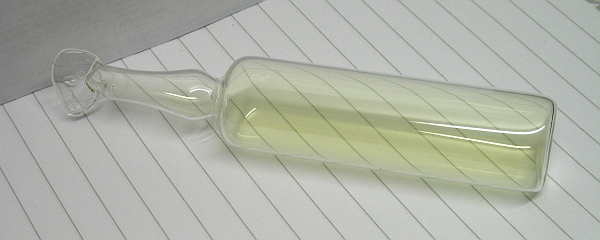
\includegraphics[height=2.9cm]{images/book2/chlorine.jpg}\hspace{0.5em}%
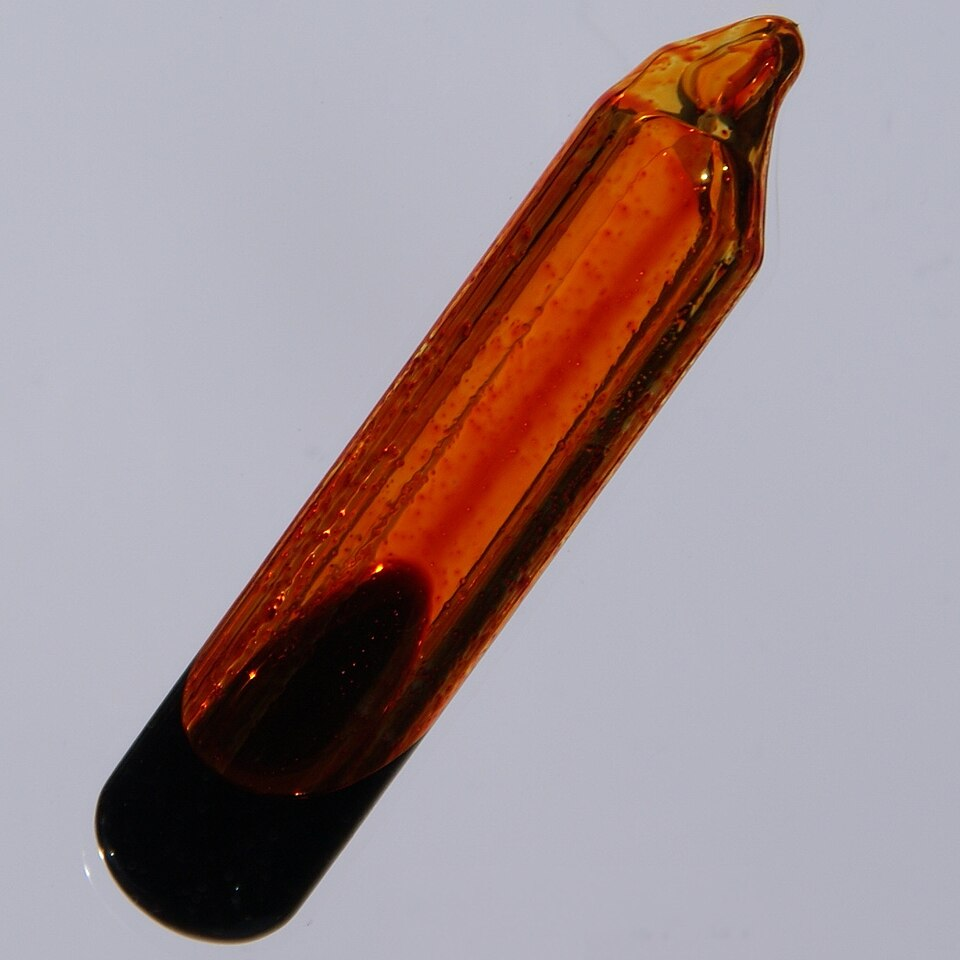
\includegraphics[height=2.9cm]{images/book2/bromine.jpg}\hspace{0.5em}%
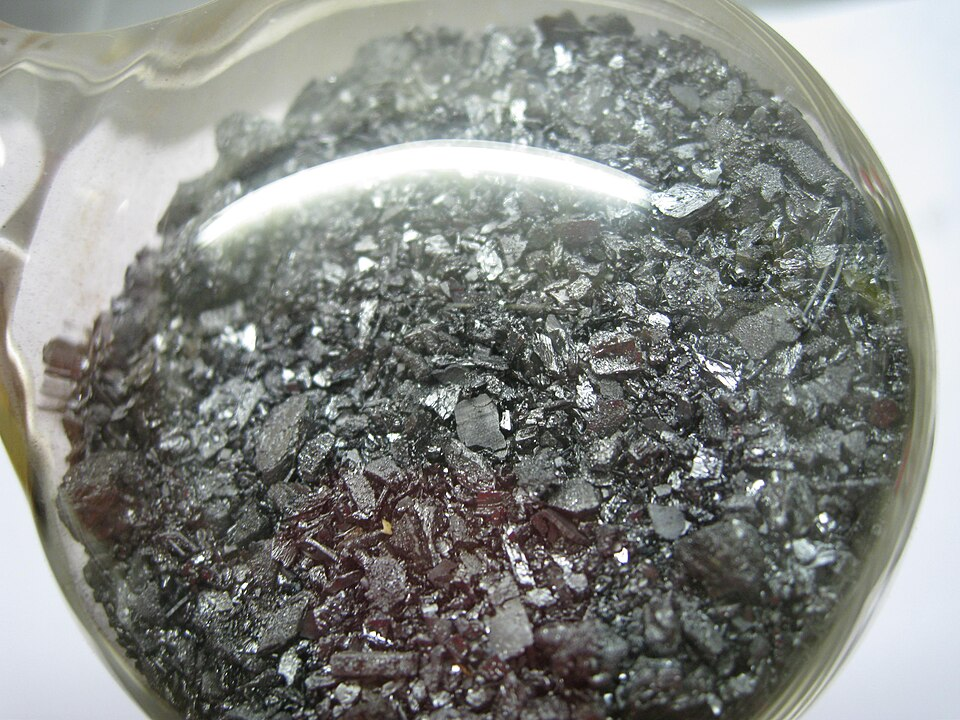
\includegraphics[height=2.9cm]{images/book2/iodine.jpg}

{\small الكلور، غاز أصفر مخضر شاحب (ف. أولن، CC BY-SA 3.0)؛
البروم، سائل أحمر داكن ببخار برتقالي (يوري، CC BY 3.0)؛ واليود،
بلورات رمادية سوداء ذات بريق فلزي (Dnn87، CC BY 3.0). والكلور
والبروم مختومان في أمبولات زجاجية. كلها من ويكيميديا كومنز.}
\end{omfigure}

\begin{proposition}[القدرة المؤكسدة للهالوجينات]\label{prop:b1:p-block-16-18:halogen-oxidising-order}
\omterm{def:b1:p-block-16-18:halogen}{الهالوجينات} مؤكسدات تتناقص قوتها نزولًا في \omterm{def:b1:periodicity:table}{الزمرة}:
\babelsublr{$E^\circ(\ce{F2}/\ce{F-}) = 2.89$~V}، $\ce{Cl2}/\ce{Cl-}$ \babelsublr{1.36~V}،
$\ce{Br2}/\ce{Br-}$ \babelsublr{1.08~V}، $\ce{I2}/\ce{I-}$ \babelsublr{0.53~V}. وكل \omterm{def:b1:p-block-16-18:halogen}{هالوجين} يؤكسد
أيونات الهاليد التي تحته في \omterm{def:b1:periodicity:table}{الزمرة}.
\end{proposition}

\begin{proof}
تأتي القيم من طاقات جيبس لتكوّن أيونات الهاليد
(\cref{ch:b1:nernst}). وبقاعدة غاما، يؤكسد \ce{X2} الأيون \ce{Y-} حين تكون
المزدوجة $\ce{X2}/\ce{X-}$ فوق $\ce{Y2}/\ce{Y-}$: مثلًا
\ce{Cl2 + 2Br- -> 2Cl- + Br2}، $\log K = 2(1.36 - 1.08)/0.059 = 9.5$.
ونزولًا في \omterm{def:b1:periodicity:table}{الزمرة}، تكبر الذرات، وتنخفض ألفتها لإلكترون إضافي
وإماهة أيونات الهاليد الأصغر، فينخفض الجهد معها.
\end{proof}
% ledger: dfg:F-_ao, dfg:Cl-_ao, dfg:Br-_ao, dfg:I-_ao

\begin{omfigure}
\begin{tikzpicture}
\begin{axis}[
  ybar, width=0.62\linewidth, height=5.0cm, ymin=0, ymax=3.3,
  symbolic x coords={F,Cl,Br,I}, xtick=data,
  xticklabels={\ce{F2}/\ce{F-}, \ce{Cl2}/\ce{Cl-}, \ce{Br2}/\ce{Br-}, \ce{I2}/\ce{I-}},
  ylabel={\babelsublr{$E^\circ$ (V)}}, bar width=16pt, nodes near coords,
  every node near coord/.append style={font=\scriptsize},
  tick label style={font=\small}, label style={font=\small}, enlarge x limits=0.2]
\addplot[fill=omThm!40, draw=omThm] coordinates {(F,2.89) (Cl,1.36) (Br,1.08) (I,0.53)};
\end{axis}
\end{tikzpicture}

{\small \omterm{def:b1:nernst:electrode-potential}{الجهود المعيارية} لمزدوجات الهالوجين--الهاليد عند
\qty{25}{\celsius}، المحسوبة من طاقات جيبس المجدولة: فالقدرة المؤكسدة
تنخفض بانتظام نزولًا في \omterm{def:b1:periodicity:table}{الزمرة}.}
\end{omfigure}

هاليدات الهيدروجين كلها أحماض في الماء، لكن \ce{HF} ضعيف
($\mathrm{p}K_a$ يساوي 3.16) بينما \ce{HCl} و\ce{HBr} و\ce{HI} قوية: فالرابطة
\ce{H-F} قوية جدًا وأيون الفلوريد الصغير مرتبط \omterm{def:b1:intermolecular-forces-solvents:hbond}{بروابط هيدروجينية}
قوية. والفلور أكثر العناصر كهرسلبية وأقوى
\omterm{def:b1:nernst:couple}{مؤكسد} في الجدول؛ ولا يُحصل عليه إلا بالتحليل الكهربائي.
وأحماض الكلور الأكسجينية --- تحت الكلوروز \ce{HClO}، والكلوريك \ce{HClO3}،
والبيركلوريك \ce{HClO4} --- تزداد قوة بعدد ذرات الأكسجين غير الحاملة
للهيدروجين، كما في كل الأحماض الأكسجينية (\cref{def:b1:p-block-13-15:oxoacid})؛
وقد رُسمت علاقاتها مع الكلوريد والكلور في
\cref{ch:b1:e-ph-diagrams}.
% ledger: dfg:HF_ao, dfg:F-_ao

\begin{omfigure}
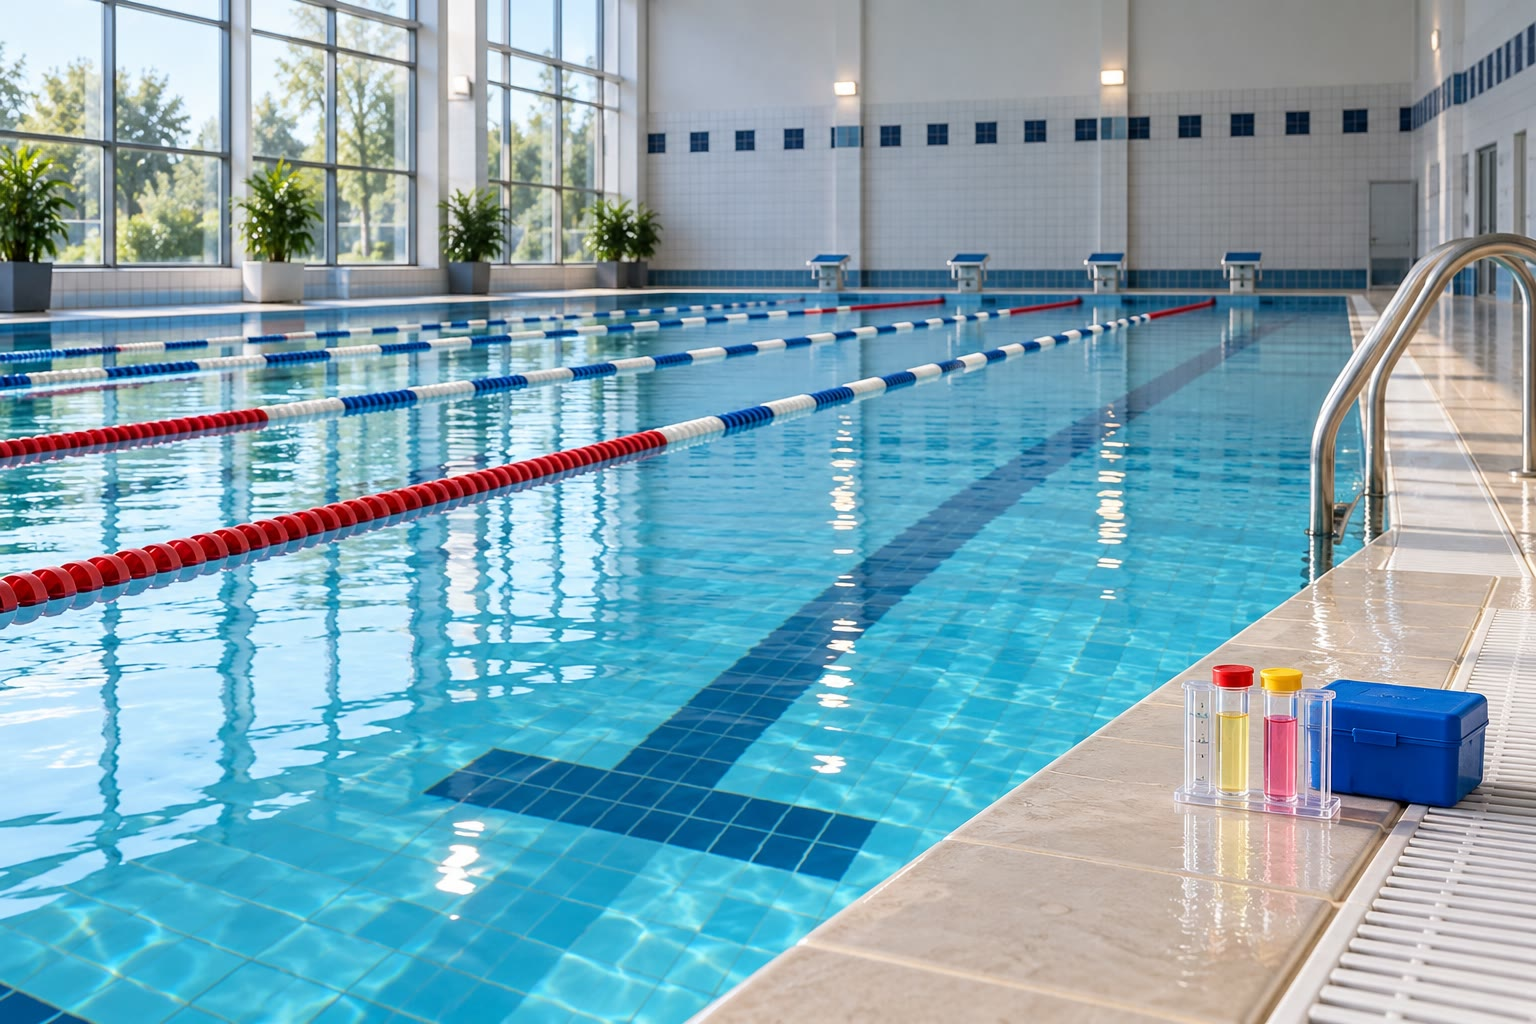
\includegraphics[width=0.55\linewidth]{images/book2/ai/b1-28-swimming-pool.jpg}

{\small مسبح عام وعدّة فحص مائه: يُفحص الكلور
المذاب على هيئة حمض تحت الكلوروز عدة مرات يوميًا.}
\end{omfigure}

\begin{definition}[المركبات بين الهالوجينية]\label{def:b1:p-block-16-18:interhalogen}
\emph{المركب بين الهالوجيني}\index{مركب بين هالوجيني} مركب
من هالوجينين مختلفين: \ce{ICl}، \ce{BrF3}، \ce{ClF3}، \ce{IF7}.
\omterm{def:b1:p-block-16-18:halogen}{والهالوجين} الأكبر والأقل كهرسلبية هو \omterm{def:b1:complexation:complex}{الذرة المركزية}، بثمانية
موسَّعة في \ce{ClF3} وما بعده.
\end{definition}

\begin{inthelab}[تداول الهالوجينات]
الكلور سام ولا يُحضَّر إلا بكميات صغيرة في خزانة
غازات؛ والبروم يحرق الجلد ويهاجم بخاره الرئتين، ولا
يُستعمل إلا مخففًا، في خزانة غازات، مع القفازات والنظارات، ومحلول ثيوكبريتات
الصوديوم في متناول اليد لهدم ما ينسكب
(\ce{4Br2 + S2O3^2- + 5H2O -> 8Br- + 2SO4^2- + 10H+}). واليود أخف
الثلاثة، لكنه يبقّع ويتسامى؛ ويُحفظ في قارورة مغلقة.
\end{inthelab}

\section{الغازات النبيلة ومركباتها}

للغازات النبيلة (He، Ne، Ar، Kr، Xe، Rn) طبقات تكافؤ ممتلئة
وأعلى طاقات تأين في دوراتها (\cref{ch:b1:periodicity}).
وقد ظُن طويلًا أنها خاملة، لكن الأثقل منها، التي إلكتروناتها الخارجية أقل
ارتباطًا، تتفاعل فعلًا مع أكثر العناصر كهرسلبية: فالزينون يعطي
\ce{XeF2} و\ce{XeF4} و\ce{XeF6} وأكاسيد. وأشكالها تتبع قواعد VSEPR
مع \omterm{def:b1:lewis-resonance-vsepr:lewis}{أزواج حرة} على الزينون.

\begin{example}[لماذا الزينون، لا الأرغون]
تنخفض طاقات التأين الأولى للغازات النبيلة نزولًا في \omterm{def:b1:periodicity:table}{الزمرة}: He
24.59، Ne 21.56، Ar 15.76، Kr 14.00، Xe 12.13، Rn \babelsublr{10.75~eV}. وطاقة تأين
ثنائي الأكسجين، \ce{O2 -> O2+ + e-}، تساوي \babelsublr{12.07~eV}، أي تكاد تساوي طاقة تأين الزينون. \omterm{def:b1:nernst:couple}{فالمؤكسد}
القوي بما يكفي لانتزاع إلكترون من \ce{O2}، فيعطي
كاتيون ثنائي الأكسجينيل \ce{O2+}، ينبغي إذن أن يؤكسد الزينون أيضًا، لا
الأرغون، الذي يتمسك بإلكترونه بقوة تزيد بمقدار \babelsublr{3.7~eV}. ويتفاعل الزينون فعلًا
مع \omterm{def:b1:nernst:couple}{المؤكسد} البالغ القوة سداسي فلوريد البلاتين \ce{PtF6}، فيعطي صلبًا
تركيبه الإجمالي \ce{XePtF6}، ومع الفلور نفسه، الذي يعطي
فلوريدات الزينون في الجدول أدناه. أما الرادون، الأسهل تأينًا، فهو
شديد الإشعاع إلى حد لا يسمح بإجراء كثير من الكيمياء عليه.
\end{example}
% ledger: ie:He, ie:Ne, ie:Ar, ie:Kr, ie:Xe, ie:Rn, ie:O2, lit:XePtF6

\begin{omfigure}
\begin{tabular}{llll}
\hline
الجزيء & الأزواج الإلكترونية حول \omterm{def:b1:complexation:complex}{الذرة المركزية} & الشكل & الزاوية المقيسة \\
\hline
\ce{SO2} & مجالان رابطان + \omterm{def:b1:lewis-resonance-vsepr:lewis}{زوج حر} واحد & منحنٍ & \ang{119.5} \\
\ce{SF6} & 6 \omterm{def:b1:lewis-resonance-vsepr:lewis}{أزواج رابطة} & ثماني الأوجه & \ang{90} \\
\ce{ClF3} & 3 \omterm{def:b1:lewis-resonance-vsepr:lewis}{أزواج رابطة} + \omterm{def:b1:lewis-resonance-vsepr:lewis}{زوجان حران} & على شكل T & \ang{87.5} \\
\ce{XeF2} & \omterm{def:b1:lewis-resonance-vsepr:lewis}{زوجان رابطان} + 3 \omterm{def:b1:lewis-resonance-vsepr:lewis}{أزواج حرة} & خطي & \ang{180} \\
\ce{XeF4} & 4 \omterm{def:b1:lewis-resonance-vsepr:lewis}{أزواج رابطة} + \omterm{def:b1:lewis-resonance-vsepr:lewis}{زوجان حران} & مربع مستوٍ & \ang{90} \\
\hline
\end{tabular}

\smallskip
{\small أشكال بعض جزيئات \omterm{def:b1:periodicity:table}{الفئة} p ذات الثمانيات الموسَّعة أو \omterm{def:b1:lewis-resonance-vsepr:lewis}{الأزواج الحرة}
(الزوايا المقيسة حيث تتوافر). وتشغل \omterm{def:b1:lewis-resonance-vsepr:lewis}{الأزواج الحرة} في \ce{XeF2}
المواضع الاستوائية الثلاثة لثنائي هرم مثلثي، فيبقى الجزيء
خطيًا.}
% ledger: geo:SO2.aOSO, geo:SF6.aFSF, geo:ClF3.aFClF, geo:XeF2.aFXeF
\end{omfigure}

الأرغون، الذي يشكّل نحو واحد بالمئة من الهواء، يحمي المواد النشطة في المختبرات
واللحام؛ والهيليوم، المستخرج من الغاز الطبيعي، يبرّد المغانط فائقة الموصلية، مثل
مغانط مطيافات الرنين المغناطيسي النووي (\cref{ch:b1:structure-spectroscopy}).
% ledger: air:Ar

\section{تمارين}

\begin{exercise}[$\star$]\label{exo:b1:p-block-16-18:1}
أعطِ \omterm{def:b1:nernst:oxidation-number}{عدد أكسدة} الكبريت في \ce{H2S}، و\ce{S8}، و\ce{SO2}،
و\ce{SO3^2-}، و\ce{SO4^2-}، و\ce{S2O3^2-} (في المتوسط) و\ce{H2S2O7}.
\end{exercise}

\begin{exercise}[$\star$]\label{exo:b1:p-block-16-18:2}
أي هذه التفاعلات يحدث: الكلور مع يوديد البوتاسيوم؛ واليود مع
بروميد الصوديوم؛ والبروم مع كلوريد الصوديوم؛ والكلور مع بروميد الصوديوم؟
اكتب التفاعلات التي تحدث.
\end{exercise}

\begin{exercise}[$\star$]\label{exo:b1:p-block-16-18:3}
ارسم \omterm{def:b1:lewis-resonance-vsepr:lewis}{بنى لويس} للجزيئات \ce{SO2} و\ce{SO3} و\ce{O3}، مع
\omterm{def:b1:lewis-resonance-vsepr:resonance}{بنى الرنين} لها، وأعطِ أشكالها.
\end{exercise}

\begin{exercise}[$\star$]\label{exo:b1:p-block-16-18:4}
اكتب تفاعلات \ce{SO2} و\ce{SO3} مع الماء ومع هيدروكسيد
الصوديوم.
\end{exercise}

\begin{exercise}[$\star\star$]\label{exo:b1:p-block-16-18:5}
احسب pH لمحلول حمض الهيدروفلوريك تركيزه \qty{0.10}{mol/L} وقارنه
بحمض الهيدروكلوريك بالتركيز نفسه. وفسّر الفرق.
\end{exercise}

\begin{exercise}[$\star\star$]\label{exo:b1:p-block-16-18:6}
توقّع \omterm{def:b1:lewis-resonance-vsepr:vsepr}{بنموذج VSEPR} أشكال \ce{BrF5}، و\ce{IF7} (سبعة \omterm{def:b1:lewis-resonance-vsepr:lewis}{أزواج رابطة}،
ثنائي هرم خماسي)، و\ce{ICl4-} و\ce{XeO3}.
\end{exercise}

\begin{exercise}[$\star\star$]\label{exo:b1:p-block-16-18:7}
احسب ثابت التفاعل \ce{Cl2 + 2I- -> 2Cl- + I2} وبيّن لماذا يحوّل ماء
الكلور ورق النشا--اليوديد إلى الأزرق.
\end{exercise}

\begin{exercise}[$\star\star$]\label{exo:b1:p-block-16-18:8}
بيّن أن الأوزون يستطيع أكسدة أيونات اليوديد إلى اليود واكتب التفاعل في
الوسط الحمضي. ولماذا يُستعمل هذا لقياس الأوزون؟
\end{exercise}

\begin{exercise}[$\star\star$]\label{exo:b1:p-block-16-18:9}
يفحّم حمض الكبريتيك المركّز السكروز، \ce{C12H22O11}. اكتب
\omterm{def:b1:alcohol-activation:dehydration}{نزع الماء} إلى الكربون واحسب كتلة الكربون من \qty{10.0}{g} من
السكر.
\end{exercise}

\begin{exercise}[$\star\star\star$]\label{exo:b1:p-block-16-18:10}
احسب pH لمحلول حمض الكبريتيك تركيزه \qty{0.10}{mol/L}، آخذًا الحمضية الثانية
في الحسبان ($\mathrm{p}K_a = 1.99$). وكم تضيف الحمضية
الثانية؟
\end{exercise}

\begin{exercise}[$\star\star\star$]\label{exo:b1:p-block-16-18:11}
مستعينًا بالجهود، فسّر لماذا لا يمكن تحضير الفلور بأكسدة
الفلوريد بأي \omterm{def:b1:nernst:couple}{مؤكسد} كيميائي في الماء، ولماذا يجب صنعه بالتحليل
الكهربائي لفلوريد منصهر، لا لمحلول مائي.
\end{exercise}

\begin{exercise}[$\star\star\star$]\label{exo:b1:p-block-16-18:12}
اليود قليل الذوبان في الماء لكنه يذوب في محلول يوديد البوتاسيوم
على هيئة أيون ثلاثي اليوديد \ce{I3-}. مستعملًا طاقات جيبس للتكوّن لكل من
\ce{I2(aq)} ($\Delta_f G^\circ = \qty{16.40}{kJ/mol}$)، و\ce{I-} ($-51.57$)
و\ce{I3-} ($-51.4$)، احسب ثابت التفاعل \ce{I2 + I- <=> I3-}.
\end{exercise}

\section{مسألة: طن واحد من الكبريت}

\begin{problem}[{مسألة نهاية الأسبوع --- حرق الكبريت، والأكسدة الحفزية
لثنائي أكسيد الكبريت، والامتصاص والأوليوم، والحمضية الثانية
لحمض الكبريتيك، وكتلة الحمض المصنوع من طن واحد من الكبريت}]
\label{pb:b1:p-block-16-18:1}
يحرق مصنع لحمض الكبريتيك كبريتًا مسترجعًا من الغاز الطبيعي. الكتل المولية
(\unit{g/mol}): S 32.1، \ce{O2} 32.0، \ce{SO2} 64.1، \ce{SO3} 80.1،
\ce{H2SO4} 98.1، \ce{H2O} 18.0؛ ويحتوي الهواء \qty{21}{\percent} من
\ce{O2} حجميًا؛ $\mathrm{p}K_a(\ce{HSO4-}) = 1.99$؛ $R =
\qty{8.314}{J/(K.mol)}$.

\medskip
\noindent\textbf{الجزء الأول --- حرق الكبريت.}
\begin{enumerate}
  \item أعطِ \omterm{def:b1:nernst:oxidation-number}{عدد أكسدة} S في S و\ce{SO2} و\ce{SO3}
        و\ce{H2SO4}.
  \item اكتب احتراق الكبريت.
  \item ارسم \omterm{def:b1:lewis-resonance-vsepr:lewis}{بنية لويس} للجزيء \ce{SO2} وتوقّع شكله.
  \item احسب كمية الكبريت في طن واحد.
  \item احسب حجم الهواء (\qty{25}{\celsius}، \qty{1}{bar}) اللازم
        للاحتراق وحده.
  \item لماذا يُبرَّد الغاز الخارج من الحارق قبل المحوِّل؟
\end{enumerate}

\medskip
\noindent\textbf{الجزء الثاني --- الأكسدة الحفزية.}
\begin{enumerate}[resume]
  \item اكتب أكسدة \ce{SO2} إلى \ce{SO3}.
  \item ثابتها عند \qty{25}{\celsius} نحو $10^{24.8}$. فلماذا يلزم
        \omterm{def:b1:elementary-steps:catalyst}{حفّاز} مع ذلك؟
  \item ما دور أكسيد الفاناديوم(V)، بلغة
        \cref{ch:b1:elementary-steps}؟
  \item ارسم شكل \ce{SO3}.
  \item لماذا يُستعمل فائض من الهواء؟
  \item ما كسر \ce{SO2} المفقود إذا كانت نسبة التحول
        \qty{99.7}{\percent}؟
\end{enumerate}

\medskip
\noindent\textbf{الجزء الثالث --- الامتصاص.}
\begin{enumerate}[resume]
  \item اكتب امتصاص \ce{SO3} في حمض الكبريتيك.
  \item لماذا لا يُمتص \ce{SO3} مباشرة في الماء؟
  \item اكتب تخفيف الأوليوم.
  \item اكتب المعادلة الإجمالية للطريقة.
  \item احسب كتلة الماء المستهلكة لكل طن من الكبريت.
  \item لماذا يجب صب الحمض في الماء وليس العكس أبدًا؟
\end{enumerate}

\medskip
\noindent\textbf{الجزء الرابع --- الحمض.}
\begin{enumerate}[resume]
  \item احسب pH لمحلول حمض الكبريتيك تركيزه \qty{0.050}{mol/L}
        مع أخذ الحمضية الثانية في الحسبان.
  \item احسب كتلة حمض الكبريتيك \omterm{def:b1:extent-q-and-k:fractional-extent}{لمردود} إجمالي قدره \qty{99.5}{\percent}.
  \item أنتج العالم نحو \qty{84}{Mt} من الكبريت سنة 2025. فما
        كتلة حمض الكبريتيك التي كان سيعطيها لو حُوّل كله؟
  \item اذكر كتلة حمض الكبريتيك الممكن الحصول عليها من طن واحد من
        الكبريت (تحول تام).
\end{enumerate}
\end{problem}
